\chapter{Guidelines}
\label{chap:guidelines}
\addtocontents{toc}{\protect\setcounter{tocdepth}{1}}

In this chapter, we present the guidelines proposed in this master thesis based on results from the Systematic Literature Review and Grounded Theory. Section \ref{sec:guidelines-overview} presents an overview of guideline structure. The next sections (\ref{sec:guidelines-G1}, \ref{sec:guidelines-G2}, \ref{sec:guidelines-G3}, \ref{sec:guidelines-G4}, \ref{sec:guidelines-G5}) present the guidelines one by one in the structure presented in Section \ref{sec:guidelines-overview}.

\section{Overview}
\label{sec:guidelines-overview}

The analysis of all data extracted shows the necessity of some rules to follow when conducting an experiment in the context of this study. The methodology used to reach the Guidelines is based on evidence by using Systematic Literature Review and Grounded Theory. The Systematic Literature Review retrieved information about the experiments executed in this area and gave us information about how the experiments are commonly applied. The Grounded Theory deepened in this information which made possible to compare what happens and what is recommended by the literature.



The five guidelines are: \nameref{sec:guidelines-G1}, \nameref{sec:guidelines-G2}, \nameref{sec:guidelines-G3}, \nameref{sec:guidelines-G4}, \nameref{sec:guidelines-G5}). The appendix \ref{ap:guidelines} presents an overview of each guidelines in the form of an infographic. An overview of the guidelines  Following some examples used in software engineering \cite{Kappel2006DevelopingMenus,Kitchenham2002PreliminaryEngineering}, we came up with the guidelines structure to evaluate the cognitive impact composed of seven parts, described as follows:
    \begin{enumerate}
        \item \textbf{When:}  In this part, we explain in which step this guideline can help. The steps are based on the five phases and steps of the experimental process described by \citeonline{Wohlin2000}.
        \item \textit{\textbf{Why:} In this part, we explain the guideline based on the scientific literature on Cognitive Psychology and Experimentation in Software Engineering.
        \item \textbf{How:} In this part, we explain how to apply the guideline in detail.
        \item \textbf{Example} In this part, we present a real example of a paper retrieved from the Systematic Literature Review.
        \item \textbf{Priority:}} In this part, we give a priority note (from 0 to 5) according to the importance of the guideline and with the problems that were found in the experiments studied.
        \item \textbf{Findings:} In this part, we present the main findings from our methodology (Systematic Literature Review and Grounded Theory) that have led to that guidelines.
        \item \textbf{Attachments:} It is an optional part where we show some graph or table to guide the rules presented.
    \end{enumerate}


\section{\textit{G1} - Specify the Hypotheses}
\label{sec:guidelines-G1}

\noindent \textit{\textbf{When:}}  In the Planning phase of the experiment process, in the Hypothesis Formulation step.
\vspace{5mm}


\noindent \textit{\textbf{Why:}} In the context of cognitive impact evaluation of multimodal interfaces for people who are blind, the experiments assume the technologies used has a cognitive impact on its users. This theory should be tested to see if it has the power to predict certain aspects of the phenomena with which it deals. Thus, the hypothesis has to be stated clearly since the Scoping phase. Even if particular findings appear to confirm a given hypothesis, the findings must be subjected to statistical analysis to determine their statistical significance and to retain or reject hypotheses \cite{Sternberg2011}. In addiction, \citeonline{Kitchenham2002PreliminaryEngineering} presents the shallow hypotheses concept, when the hypothesis is simply a statement of the tests to be performed, thus it does not reflect an underlying, explanatory theory. This represents the care that must be taken in the decision.
\vspace{5mm}

\noindent \textit{\textbf{How:}} Two kinds of hypotheses have to be formulated: a null hypothesis, states that there are no real underlying trends or patterns in the experiment setting; and alternative hypotheses, that are the hypotheses in favor of which the null hypothesis is rejected.  Choose one statistical test to evaluate the outcome of an experiment. More commonly, however, researchers use various statistical means of analyzing the data \cite{Sternberg2011}. The description of both null and alternative hypotheses should be as formal as possible \cite{Jedlitschka2007}.
%Table X\todo{} presents the most common statistical methods. 
\vspace{5mm}

\noindent \textit{\textbf{Example:}} The study ``Navigational 3D audio-based game-training towards rich auditory'' \cite{Balan2014} works with the hypothesis that the occipital visual cortex is not completely visual and that it shares functionality with other perceptual modalities. The researchers had used the Student t-test as a statistical method to test the hypothesis. As a result, the paired average from experiments proved to be non-significant (p=0.3 at p<0.01), and they reject the null hypothesis. These results lead to the hypothesis that the players could have rendered the audio data into a visual, imaginary representation of the virtual setting.
\vspace{5mm}

\noindent \textit{\textbf{Priority:}} 5/5
\vspace{5mm}

\noindent \textit{\textbf{Findings:}} Only 11 experiments from 52 experiments retrieved presented the hypothesis of the experiment in the text, among them, only 4 presented well, as a specific section to show the hypothesis or showed the null hypothesis beyond the general purpose of the study.
\vspace{5mm}

\section{\textit{G2} - Define and report the experiment variables}
\label{sec:guidelines-G2}

\noindent \textit{\textbf{When:}} 
In the Planning phase of the experiment process, in the Variable Selection step, and in the Presentation \& package phase.
\vspace{5mm}

\noindent \textit{\textbf{Why:}} In any controlled experimental designs, the variables should relate to many cognitive aspects of the experimental situation are controlled. There are two kinds of variables need to be described: dependent and independent variables. Independent variables are those variables that we manipulate in the experiment to see the factors influence in the phenomena \cite{Wohlin2000}, while other aspects of the investigation are held constant (control variables). Dependent variables are outcome responses, the values of which depend on how one or more independent variables influence or affect the participants in the experiment \cite{Sternberg2011}. Often there is only one dependent variable, and it should, therefore, be derived directly from the hypothesis \cite{Wohlin2000}.

Different from Software Engineering literature, the Cognitive Psychology evaluation process insert a new concept, the irrelevant variables. The confounding variables are a type of irrelevant variable that has been left uncontrolled in a study. When conducting research, we must be careful to avoid the influence of confounding variables. Treatment is one particular value of an independent variable manipulated. When the experimenter manipulates the independent variables, he or she controls for the effects of irrelevant variables and observes the effects on the dependent variables (outcomes). These irrelevant variables that are held constant are called control variables \cite{Sternberg2011}. 

In the context of cognitive evaluation and based on systematic literature review findings, we present the merge of these two approaches in Figure \ref{fig:central_idea_of_cognitive_impact2}.

	\begin{figure}[h] 

   	    \captionsetup{width=10cm}%Da mesma largura que a figura
		\Caption{\label{fig:central_idea_of_cognitive_impact2} Relation between variables}
		\UFCfig{}{
			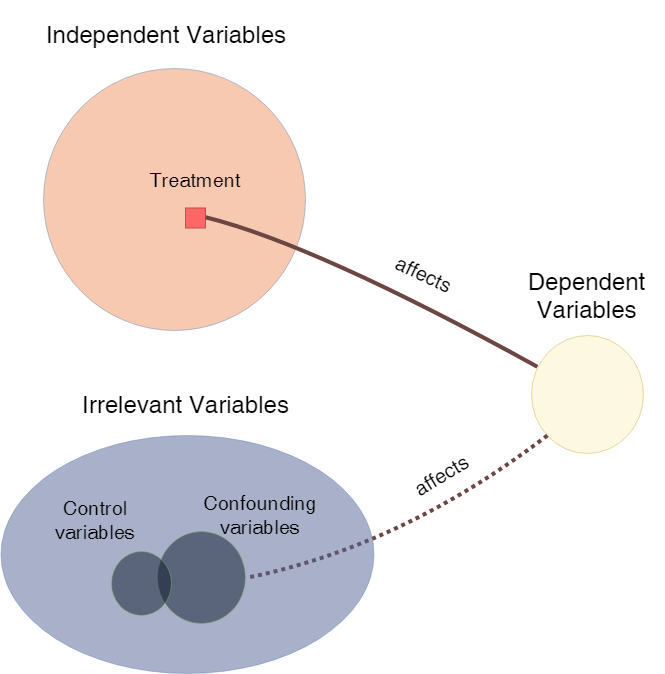
\includegraphics[width=10cm]{figuras/central_idea_of_cognitive_impact2.png}
		}{
			\Fonte{Produced by the author.}
		}	
	\end{figure}
\vspace{5mm}

\noindent \textit{\textbf{How:}} First, the variables must be understood and defined in the planning phase. We recommend the classification proposed above that is clear about the type of variable. Despite it is most important to select variables following the purpose of the experiment, the Variables code map (see Figure \ref{fig:variables__code_map}) presents a range of possible variables. Use this range to guide through the choice.

It is essential not only to identify appropriate contextual variables but also to measure them consistently \cite{Kitchenham2002PreliminaryEngineering}. The Measures code map (see Figure \ref{fig:measures_code_map}) presents a range of possible measures. To measure, check specific instruments in the literature that have already been used before. There are several surveys, checklists, checklists, questionnaires, kits and logs used in literature and the uses of published instruments turns the experiment more rigor. In the attachments of this guideline, we present a practical example of how to describe the variables in the experiment. Building a pattern for results provides a consistent basis for comparing and classifying cognitive impact.
\vspace{5mm}

\noindent \textit{\textbf{Example:}} The study ``Construction of cognitive maps of unknown spaces using a multisensory virtual environment for people who are blind''\cite{Lahav2008b} defines the experiment as follow:
\begin{description}
    \item[Dependent Variable] Navigation performance (relate to the participants’ cognitive map of the explored space):
    
   \begin{enumerate}[label=\alph*.]
       \item	cognitive map structural components: Eight variables related to the cognitive map structural components referred to the accurate mapping of spatial structure information.
       \item	spatial relationships estimation: (1) references creation, (2) directions estimation, and (3) distances estimation.
       \item	cognitive map construction process: Spatial strategy, Spatial model used, Chronology of the descriptive process 
   \end{enumerate}
   
   \item[Independent Variable] level of blindness, gender, age, Maps abilities, language spoken, onset of blindness, assistive aid, other disabilities.
   
   \item[Factor] Experimental group (21 participants) x control group (10 participants), type of environment explored (the MVE and the real space).
   
\end{description}

Eight variables related to the cognitive map structural components referred to the accurate mapping of: (1) room size, (2) room shape, (3) structural components (e.g., doors, windows), (4) structural component location, (5) objects within the room (e.g., boxes, cubes), (6) object location, (7) object size, and (8) object position. Three variables were related to spatial relationships estimation: (1) references creation (e.g., landmarks, spatial relations – behind, nearby), (2) directions estimation (e.g., to the north, room’s center), and (3) distances estimation (e.g., close-to, steps).

The study defines two groups that were similar in gender, age, and age of vision loss (congenitally blind or late-blind). The experimental group included 21 participants who explored the unknown space by means of the MVE. The control group included 10 participants who explored the unknown space by actual navigation in the real space.
\vspace{5mm}

\noindent \textit{\textbf{Priority:}} 5/5

\noindent \textit{\textbf{Findings:}} In cognitive impact experiments, the dependent variables are related to performance or cognitive skills, and some of them works with user emotions as dependent variables.

%11 experiments have their variables well described in a separated section in the text. 8 experiments work with a control group to compare with the treatment.

% we produce three categories of dependent variables and three categories of independent variables. In searching this, we can see the variables are strongly related to the experiment hypothesis or objective when the hypotheses are not explicit in the text.
 
\vspace{5mm}

\noindent \textbf{Attachments:} Table \ref{tab:schema_for_description_of_variables} presents schema to describe the variables. The name of the variable could have a code to be referenced later. The type of the variable could be independent, dependent, irrelevant or more detailed as shown in Figure \ref{fig:central_idea_of_cognitive_impact2}. The abbreviation could be a simple name from the hole name. The variables can be divided into three different classes: product, process, and resource. The process describes which activities that are needed to produce the software. The products are the artifacts, deliverables or documents that results from a process activity. Resources are the objects, such as personnel, hardware, or software, needed for a process activity \cite{Wohlin2000}. The entity is the instance of the class. The type of attribute could be internal, that can be measured purely in terms of the object, or external, that can only be measured with respect to how the object relates to other objects. The scale type could be nominal, ordinal and others. Beyond the scale type, the table presents the unit and the range for nominal and restricted ordinal scales it should present the definition of each scale point. And finally the counting rule in the context of the entity.
%%%%%Comentário do .doc%%%%
%refazer um próprio com foco no tipo de avaliação prevista%

\begin{table}[h]
	\captionsetup{width=16cm}%Deixe da mesma largura que a tabela
	\Caption{\label{tab:schema_for_description_of_variables} Schema for description of variables}%
	\IBGEtab{}{%
		\begin{tabular}{m{1.3cm}m{1.5cm}m{1.3cm}m{1.2cm}m{1cm}m{1.3cm}m{1.1cm}m{.5cm}m{1.7cm}m{1cm}}
			\toprule
		    Name of the variable & Type of the variable & Abbreviation & Class & Entity & Type of attribute & Scale type & Unit & Range & Counting rule \\
%			\midrule \midrule
			\bottomrule 
		\end{tabular}%
	}{%
	\Fonte{Adapted from \citeonline{Jedlitschka2007}.}%
%	\Nota{esta é uma nota, que diz que os dados são baseados na	regressão linear.}%
%	\Nota[Anotações]{uma anotação adicional, seguida de várias outras.}%
    }
    \end{table}
%%%% figura excluida e comentada %%%%
\begin{comment}
	\begin{figure}[h] 

   	    \captionsetup{width=16cm}%Da mesma largura que a figura
		\Caption{\label{fig:schema_for_description_of_variables} Schema for description of variables }
		\UFCfig{}{
			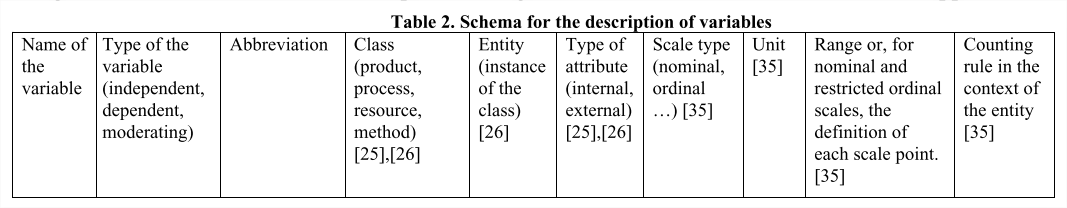
\includegraphics[width=16cm]{figuras/schema_for_description_of_variables.png}
		}{
			\Fonte{Adapted from \citeonline{Jedlitschka2007}.}
		}	
	\end{figure}
\end{comment}
\vspace{5mm}

\section{\textit{G3} - Choose a valid sample}
\label{sec:guidelines-G3}

\noindent \textit{\textbf{When:}}  
In the Planning phase of the experiment process, in the Hypothesis Formulation step. 
\vspace{5mm}

\noindent \textit{\textbf{Why:}} The selection of subjects, also called a sample, is closely connected to the generalization of the results from the experiment. With the objective of generalizing the results to the desired population, the selection must be representative of that population \cite{Kitchenham2002PreliminaryEngineering}. \citeonline{Wohlin2000} presents two sampling categories, the probability, and the non-probability, and give three examples from each sampling techniques. Among these examples, the most sample encountered in the impact experiments in the context of this work are Simple random sampling (subjects are selected from a list of the population at random) and Convenience sampling (the nearest and most convenient persons are selected as subjects). Other examples could be read in \citeonline{Wohlin2000}.

The size of the sample also impacts the generalization of the results. The size of the sample affects the error rate, and it is closely related to the power of the statistical test \cite{Wohlin2000}. Wohlin presents some general principles for choosing the sample size:

\begin{quotation}
     If there is significant variability in the population, the larger sample size is needed. And the analysis of the data may influence the choice of the sample size.
\end{quotation}

Moreover, all participant characteristics that might have an effect on the results or restrict the sample in some way should be well described in the experiment report \cite{Jedlitschka2007}. For the subjects who are blind or visually impaired, the following characteristics must take account in the sampling selection, and in the report: blindness level, blindness onset, and etiology of blindness.

Concerning the blindness level, there are many definitions about it. In general, the experiments use the categories of ``Blindness and Deafness'' \cite{WHO2018Blindness}. This institution defines two categories: blind and visually impaired. Different from this concept of the blind, some papers call the participants as legally blind, which depends on the country laws and are broader than blind (see Section \ref{subsec:background-blindness}). Some of the experiments present blindfolded participants or even blindfolded the visually impaired participants to equal the visual acuity. The participation of sighted blindfolded subjects is interesting to compare results; however, this set does not present the real perception of a blind subject, mainly in cognitive aspects.
%TODO encontrar essa referência

The blindness onset (the time with impairment) and its etiology are characteristics that should take into account because this could affect the results.  Given the enormous variety of possible combinations with these characteristics, most of the papers report the characteristics and assume as threats to validity. Confounding variables touching these characteristics could be controlled in the sampling choice.

The sample selection may include experience with the technology or mean/range of experience in years, or educational level \cite{Shull2008GuideEngineering}. Concerning a skill of subjects, a good approach has used a pre-test to capture the experience and divide the subjects into groups. 

In the experiment report, the sampling strategy and the resulting samples need to be described, including the number of participants (per condition), the kind of participants (e.g., computer science students), and the populations from which they were drawn \cite{Jedlitschka2007}.
\vspace{5mm}

\noindent \textit{\textbf{How:}} In the planning phase, experimenters must plan to use a representative sample of the population of interest. In this point, there are the following topics.
\begin{enumerate}
    \item \textbf{Number of users:} choose as larger as possible in resources available and preferably the size no less than 6 persons This number is grounded evidence-based information from the Systematic Literature Review where most of the experiments have presented from 6 to 10 participants.
    \item \textbf{Blindness level distribution:} choose the blindness level distribution according to the variables of the experiment. Do not use only sighted blindfolded participants, since they do not represent the cognitive perception of a blind person. However, if the visual feedback is significant to accomplish the task, when possible, blindfold all participants to equal the visual acuity. When there are sighted persons, balance the number of sighted and blind participants.
    \item \textbf{Sampling technique:} prioritize the use of simple random sampling.
\end{enumerate}
    %\item \textbf{Gender information:} We suggest balancing in the sample the number of each gender, female and male.
    %\todo{RETIRADO Gender information We suggest balancing in the sample the number of each gender, female and male.}

All this information needs to be described in detail. We suggest putting all information in a table careful to not identify the participants. Do not forget the age, gender and blindness level.
\vspace{5mm}

\noindent \textit{\textbf{Example:}} The study ``Assessment of feedback modalities for wearable visual aids in blind mobility''\cite{Adebiyi2017} has a sample with 23 users, among them 12 are blind, and 11 are visually impaired. They present in each blindness level group the gender and the age range. Moreover, the experiment reports a table with code, age, gender and diagnosis of Vision Loss. 
\vspace{5mm}

\noindent \textit{\textbf{Priority:}}  4/5
\vspace{5mm}

\noindent \textit{\textbf{Findings:}} One experiment does not inform the number of users. Moreover, 7 experiments do not inform the age of participants. The majority of experiments works with convenience sampling. We suppose that this happens because the kind of population involved, which is restricted to people who are blind or visually impaired. 9 experiments do not inform the proportions of the blind, low vision, sighted and blindfolded. 16 experiments do not inform the gender distribution. Gender is equilibrated. Only 3 experiments have used random groups.
\vspace{5mm}

\section{\textit{G4} - Plan and Report Ethical Concepts}
\label{sec:guidelines-G4}
\vspace{5mm}

\noindent \textit{\textbf{When:}}  
In the Planning phase of the experiment process, in the Selection of Subjects step and the Presentation \& package phase.
\vspace{5mm}

\noindent \textit{\textbf{Why:}} In contrast, the ethical issues raised by empirical methods have received little attention in the software engineering literature \cite{Vinson2008AHumans}. Any empirical research activity involving human subjects must consider ethical aspects \cite{Wohlin2000}.  Based on \cite{Vinson2008AHumans}  the experiment must have:
\begin{itemize}
    \item \textbf{Ethical review:} Legislation of some countries requires an ethical review for studies involving human subjects. Some types of study in Software Engineering do not need to have an ethical review, but in the context of Cognitive Impact, the experiment should have an ethical review.
    \item \textbf{Informed consent:} The basis for a human-oriented empirical study (e.g., an experiment) is that subjects are participating voluntarily and that they have enough information to decide to participate or not.
    \item \textbf{Confidentiality:} The subjects must be sure that any information they share with researchers will remain confidential, which includes data privacy, data anonymity, and anonymity of participation. The researchers must lead to publishing their results without harming the companies’ and individuals’ integrity.
    \item \textbf{Sensitive results:} Outcomes from an empirical study may be sensitive in different respects for different stakeholders, that should be participants and institutions, as universities or enterprises involved.
    \item \textbf{Inducement:} In recruiting subjects for an experiment, there must be inducements to motivate their participation. However, the value should not be too large, since this could cause people to participate merely to receive the inducement.
    \item \textbf{ Feedback:} To maintain long-term relationships and trust with the subjects of a study, feedback of results and analysis are important.
    
\end{itemize}
\vspace{5mm}

\noindent \textit{\textbf{How:}} The experimenters must have to look at the ethical concepts when preparing the subjects groups. First, send the ethical review to the institution responsible in your jurisprudence. When calling a participant, present the informed consent to sign. Remember that the consent must be read to a participant who is blind, and he/she should sign with a witness, if the consent is not accessible, such as on printed paper. Take care of the sensitive results, following the procedures approved in the ethical review. Do not forget citing the ethical review and informed consent when reporting.
\vspace{5mm}

\noindent \textit{\textbf{Example:}} The study ``Virtual environments for the transfer of navigation skills in the blind: a comparison of directed instruction vs. video game based learning approaches'' \cite{201449} presents the stop rules for enforcing ethical concept, written consent, and procedures approved by the Massachusetts Eye and Ear Infirmary.
\vspace{5mm}

\noindent \textit{\textbf{Priority:}} 5/5
\vspace{5mm}

\noindent \textit{\textbf{Findings:}} 9 experiments express some information concern the ethical concepts. They explain Signing consent forms (8), stop rules (2), institutions approval (6) and user safety (2).
\vspace{5mm}

\section{\textit{G5} - Specify the resources available to all parties involved}
\label{sec:guidelines-G5}

\noindent \textit{\textbf{When:}}  
In the Planning phase of the experiment process, in the Context Selection step and the Presentation \& package phase.
\vspace{5mm}

\noindent \textit{\textbf{Why:}} In software development organizations, methods and tools are employed that frequently lack sufficient evidence regarding their suitability, limits, qualities, costs, and associated risks \cite{Vinson2008AHumans}. Regarding this, the experiment must be clear about their resources and how it leads to threats of validity. \citeonline{Jedlitschka2007} say to describe the impacts with regard to cost, schedule, and quality, circumstances under which the approach presumably will not yield the expected benefit.
\vspace{5mm}

\noindent \textit{\textbf{How:}} In the Context Selection step, the researchers should plan the time, human resources and costs available. In the Presentation and Package phase, the researcher should explain when the experiment occurs and how long are the execution of the whole or each stage. The costs are interesting mainly when the participants receive money because it could impact the experiment.
\vspace{5mm}

\noindent \textit{\textbf{Example:}} The study ``Timbremap: Enabling the Visually-Impaired to Use Maps on Touch-Enabled Devices'' \cite{Su2010} works present the scheduled for evaluating session (3-hour), and honorarium for their time granted for participants (\$60).
\vspace{5mm}

\noindent \textit{\textbf{Priority:}} 2/5
\vspace{5mm}

\noindent \textit{\textbf{Findings:}} 19 experiments describe some information about the resource, as time or costs. Only 4 experiments explain some information about cost. 1 experiment says pay \$25 per hour to participants; other pays \$60 for 3-hour sessions. 1 paper describes their team to apply the experiment.
\vspace{5mm}